\documentclass[10pt,letterpaper]{article}

\usepackage[T1]{fontenc}
\usepackage[utf8]{inputenc}
\usepackage{newtxtext}
\usepackage{newtxmath}
\usepackage[margin=0.76in,top=0.78in,bottom=0.78in]{geometry}
\usepackage{amsmath,mathtools}
\usepackage{microtype}
\usepackage{graphicx}
\usepackage{booktabs}
\usepackage{array}
\usepackage{tabularx}
\usepackage{multirow}
\usepackage[table]{xcolor}
\usepackage{enumitem}
\usepackage{fancyhdr}
\usepackage{titlesec}
\usepackage{placeins}
\usepackage[numbers,sort&compress]{natbib}
\usepackage[colorlinks=true,linkcolor=navy,citecolor=navy,urlcolor=navy]{hyperref}

\definecolor{navy}{HTML}{1B4F72}
\definecolor{tealdark}{HTML}{145A32}
\definecolor{greenbg}{HTML}{EAFAF1}
\definecolor{reddark}{HTML}{922B21}
\definecolor{redbg}{HTML}{FDEDEC}
\definecolor{amberdark}{HTML}{7D6608}
\definecolor{amberbg}{HTML}{FEF9E7}
\definecolor{slate}{HTML}{34495E}
\definecolor{lightgray}{HTML}{F4F6F7}
\definecolor{bordergray}{HTML}{BDC3C7}

\titleformat{\section}{\large\bfseries\color{navy}}{\thesection.}{0.55em}{}[\vspace{-0.4em}\color{bordergray}\rule{\linewidth}{0.6pt}]
\titleformat{\subsection}{\normalsize\bfseries\color{slate}}{\thesubsection}{0.5em}{}
\titlespacing*{\section}{0pt}{13pt}{5.5pt}
\titlespacing*{\subsection}{0pt}{8.5pt}{3pt}

\pagestyle{fancy}
\fancyhf{}
\fancyhead[L]{\footnotesize\color{slate}\textsc{V15 Paper 1 Feasibility Analysis --- PVB Continuous Hilbert Frame Theory}}
\fancyhead[R]{\footnotesize\color{slate}November 2026}
\fancyfoot[C]{\footnotesize\thepage}
\renewcommand{\headrulewidth}{0.4pt}

\newcommand{\abs}[1]{\lvert #1 \rvert}
\newcommand{\norm}[1]{\lVert #1 \rVert}
\newcommand{\ket}[1]{\lvert #1 \rangle}
\newcommand{\bra}[1]{\langle #1 \rvert}
\newcommand{\braket}[2]{\langle #1 | #2 \rangle}

\begin{document}

\begin{center}
  {\LARGE\bfseries\color{navy} Feasibility Analysis of V15 Paper 1:}\\[4pt]
  {\Large\bfseries\color{slate} Continuous Hilbert Frame Theory, Paraxial Propagation Invariance, and Exact Laguerre--Gaussian Expansion of Finite-Width Perfect Optical Vortex Beams}\\[8pt]
  {\small\color{slate}
    \textbf{Author:} Sebasti\'an Ayala (ORCID: \texttt{0009-0003-7348-3883}) \quad$|$\quad
    \textbf{Baseline:} Post-APS Triage Audit of V14 (\texttt{AY13023}) \\[2pt]
    \textbf{Open-Access Library:} 14 verified arXiv PDFs downloaded; 36 clean physics/optics BibTeX entries \quad$|$\quad
    \textbf{Date:} November 24, 2026
  }
\end{center}
\vspace{4pt}

\noindent\fcolorbox{tealdark}{greenbg}{%
\begin{minipage}{\dimexpr\linewidth-2\fboxsep-2\fboxrule\relax}
\vspace{3pt}
\textbf{\color{tealdark}\large EXECUTIVE VERDICT: HIGHLY FEASIBLE (\textsc{STRONG GO} AS A STANDALONE PAPER FOR \emph{JOSA A}, \emph{J.\ OPT.}, OR \emph{J.\ PHYS.\ A})}\\[4pt]
\small
The mathematical core of V14 Part~I is sound and numerically verified to machine precision. Its $<24\,$h desk rejection by \emph{Physical Review A} (\texttt{AY13023}) resulted from preventable editorial triage flags (AI/HITL framing on page~1, 23.1\% AI-meta citation pollution, simultaneous Part~I/II companion submission, and scope mismatch with PRA) rather than flawed equations. Re-architecting Paper~1 into a \textbf{fully self-contained standalone manuscript (V15)} with four concrete scientific upgrades makes it strongly competitive for zero-APC subscription publication in top optics and mathematical-physics venues:
\begin{itemize}[leftmargin=1.4em,itemsep=2pt,topsep=3pt]
  \item \textbf{New Exact 3D Propagation Result ($[S_w, \mathcal{U}_z] = 0$):} We prove a closed-form complex-waist Fresnel propagation formula $\Phi_{l,R}^{(z)}$ with $w_c^2(z) = w^2(1 + iz/z_R^{\mathrm{ring}})$ (verified to $5.3\times 10^{-23}$ against 40-digit Hankel quadrature and $4.7\times 10^{-16}$ against 2D FFT), establishing exact $z$-invariance of the frame operator $S_w^{(z)} = S_w$ and Paley--Wiener bounds $(A, B)$, while correcting a $\sigma_m^{-1} \mapsto \sigma_m^{+1}$ dimensional-scaling typo inherited from V14 Part~II in the wavefront-compensated Gouy analyzer.
  \item \textbf{Self-Contained Theory-to-Deconvolution Loop:} Integrating the worked noisy $\mathrm{LG}_{2,1}$ Tikhonov deconvolution benchmark ($\alpha_{\mathrm{reg}}^{\mathrm{opt}} = 0.04902$, $258.6\times$ / $24.13\,\mathrm{dB}$ MSE reduction, 2D-FFT Monte Carlo $0.03488\pm 0.00013$ vs.\ Parseval $0.03481$) directly validates Proposition~2 inside Paper~1 without circular forward citations to an unpublished Paper~2.
  \item \textbf{Expanded Literature Foundation \& Solo-Author Strategy:} Removing all 6 AI-meta references and adding 14 verified open-access arXiv papers lifts physics/optics coverage from 19 to 36 references. Posting first to arXiv (\texttt{physics.optics}, building on the author's existing arXiv papers \texttt{2605.15408} and \texttt{2308.11354}) and targeting \textbf{\emph{JOSA A}} ($\le 10$ published pages, \$0 mandatory fee), \textbf{\emph{Journal of Optics}} (\$0 subscription, double-anonymous review), or \textbf{\emph{Journal of Physics A}} (\$0 subscription, double-anonymous review) neutralizes solo-author triage bias completely.
\end{itemize}
\vspace{2pt}
\end{minipage}}

\vspace{4pt}

\section{Open-Access Literature Audit and Scientific Positioning}
\label{sec:lit_audit}

A central weakness identified in our \texttt{paper-orchestra} audit of V14 Part~I was its sparse physics bibliography: only 19 of 26 references were optics/mathematics papers, while 6 (23.1\%) were AI-policy articles. For V15 Paper~1, all non-physics citations have been purged and \textbf{14 verified open-access arXiv PDFs} have been retrieved and stored in \texttt{Paper PVB/V15/Paper 1/References/} alongside a clean 36-entry database (\texttt{references\_v15\_paper1.bib}). Table~\ref{tab:p1_refs} maps the newly added open-access corpus to four concrete scientific gaps resolved by V15 Paper~1.

\begin{table}[t]
\centering
\caption{Newly curated open-access arXiv literature downloaded into \texttt{V15/Paper 1/References/} (14 verified PDFs) and its exact scientific positioning relative to V15 Paper~1.}
\label{tab:p1_refs}
\scriptsize
\renewcommand{\arraystretch}{1.16}
\begin{tabularx}{\linewidth}{@{}l>{\raggedright\arraybackslash}p{4.6cm}>{\raggedright\arraybackslash}X@{}}
\toprule
\textbf{Pillar} & \textbf{Open-Access Reference (arXiv / Journal)} & \textbf{Gap Addressed by V15 Paper~1} \\
\midrule
\multirow{4}{*}{\textbf{I. Finite-Width PVB Physics}}
  & Ferreira, Ayala \emph{et al.} (2026)~\cite{Ferreira2026} (\texttt{2605.15408}, \emph{J.\ Opt.}) & Direct predecessor: proves $w\to 0$ completeness and notes finite-$w$ Gaussian smoothing for $p=0$ only (App.~D). V15 resolves global operator inversion and all $p\ge 0$. \\
  & Pinnell \emph{et al.} (2019)~\cite{Pinnell2019HowPerfect,Pinnell2019Quantitative} (\texttt{1908.04428}, \texttt{1902.04547}, \emph{Opt.\ Lett.}) & Quantifies practical imperfections of physical PVBs. V15 explains them analytically via the $(l^2/8)(w/R)^4$ peak shift, Paley--Wiener lower bound, and radial washout limit. \\
  & Yan \emph{et al.} (2022)~\cite{Yan2022Customizable} (\texttt{2209.01723}); Jabir \emph{et al.} (2016)~\cite{Jabir2016Variable} (\texttt{1601.03129}) & Connects customizable LG--PVB synthesis and variable-size Fourier generation directly to our exact $(p+1)$-term expansion $c_{l,p}(R)$ and $2f$ bridge. \\
  & Banerji \emph{et al.} (2016)~\cite{Banerji2016} (\texttt{1603.00321}) \& Barral--Li\~nares (2017)~\cite{Barral2017} (\texttt{1710.08879}) & Debates ideal vs.\ physical optical lens transformations for quantum vortices; underscores why finite $w>0$ and finite NA $k_{\max}$ are physically indispensable. \\
\midrule
\multirow{2}{*}{\textbf{II. Radial LG Modes}}
  & Plick \& Krenn (2015)~\cite{Plick2015} (\texttt{1306.6517}, \emph{PRA}) & Establishes the physical meaning of the radial index $p$ and radial-confinement operators. \\
  & Karimi \emph{et al.} (2014)~\cite{Karimi2014} (\texttt{1401.4985}, \emph{PRA}) & Develops the $\mathfrak{su}(1,1)$ radial ladder algebra; V15 complements this by giving exact finite-width PVB frame projections $c_{l,p}(R)$ for every $p\ge 0$. \\
\midrule
\multirow{2}{*}{\textbf{III. Optical Coherent States}}
  & Gazeau (2019)~\cite{Gazeau2018} (\texttt{1810.06473}) & Reviews continuous frames and Laguerre-polynomial optical coherent states; anchors our Table comparing Dirac PVBs, physical PVBs, $\mathrm{LG}_{p,l}$, and $\ket{\alpha}$. \\
  & Morales Rodr\'iguez \emph{et al.} (2024)~\cite{MoralesRodriguez2024OL,MoralesRodriguez2024PRA} (\texttt{2310.08510}, \texttt{2406.00169}) & Constructs coherent states of LG modes; contrasts directly with PVB continuous frames (non-tight Gaussian convolution frame vs.\ tight coherent-state frame). \\
\midrule
\multirow{2}{*}{\textbf{IV. Continuous Frames}}
  & Gr\"ochenig \emph{et al.} (2016)~\cite{Grochenig2016} (\texttt{1507.02124}, \emph{J.\ Approx.\ Theory}) & Rigorous completeness and stability of Gaussian-windowed Gabor systems (paired with Bastiaans~\cite{Bastiaans1980} in optical signal analysis). \\
  & Bownik \& Jasper (2026)~\cite{Bownik2026} (\texttt{2603.10423}) & Recent 2026 theorem on uniform discretization of continuous frames, directly contextualizing our transition from continuous $S_w$ to discrete Toeplitz Gram matrices $[\gamma]_{nm}$. \\
\bottomrule
\end{tabularx}
\end{table}

\section{Quantitative Verification of Core and New V15 Paper 1 Results}
\label{sec:verification}

All mathematical claims planned for V15 Paper~1 have been independently audited in \texttt{verify\_paper1\_v15.py} (SymPy symbolic algebra, 40--50-digit \texttt{mpmath} quadrature, and $512\times 512$ 2D-FFT simulations; 7/7 test suites passed). Table~\ref{tab:p1_benchmarks} and Fig.~\ref{fig:p1_feas} summarize the verified quantitative pillars.

\begin{table}[t]
\centering
\caption{Verified analytical and numerical benchmarks for V15 Paper~1 (\texttt{verify\_paper1\_v15.py}, 7/7 suites passed).}
\label{tab:p1_benchmarks}
\scriptsize
\renewcommand{\arraystretch}{1.14}
\begin{tabularx}{\linewidth}{@{}l>{\raggedright\arraybackslash}p{4.3cm}>{\raggedright\arraybackslash}X@{}}
\toprule
\textbf{Result / Section} & \textbf{Key Formula / Metric} & \textbf{Independent Verification Status} \\
\midrule
Differential Peak Shift & $\Delta r_{\mathrm{peak}}(l) \approx \frac{l^2}{8}(w/R)^4 R$ & SymPy exact series ($c_1=-1/4, c_2=(4l^2-3)/32$); matches transcendental root within $1.2\%$ at $w/R=0.10$ ($l=1\text{--}6$). \\
Continuous Frame Operator & $S_w = G_w * \cdot$, $\widetilde{G}_w(k_\perp) = e^{-w^2 k_\perp^2/2}$ & Optimal Bessel upper bound $B=1$, sharp Paley--Wiener lower bound $A=e^{-w^2 k_{\max}^2/2}$ verified via SymPy annulus limits. \\
\rowcolor{greenbg}
\textbf{NEW:} Fresnel Propagation Invariance & $\Phi_{l,R}^{(z)} = \frac{\sqrt{2/\pi}}{w_c^2(z)} e^{il\phi} e^{-\frac{r^2+R^2}{w_c^2(z)}} I_{\abs{l}}\!\bigl(\frac{2Rr}{w_c^2(z)}\bigr)$, $[S_w,\mathcal{U}_z]=0$ & Max 40-digit Hankel quadrature rel.\ err.\ $5.27\times 10^{-23}$; 2D-FFT rel.\ $L^2$ err.\ $4.73\times 10^{-16}$; unitary inner-product err.\ $6.27\times 10^{-16}$; Gouy-analyzer err.\ $5.78\times 10^{-16}$ (fixed V14 $\sigma_m^{+1}$ bug). \\
\rowcolor{greenbg}
\textbf{INTEGRATED:} Tikhonov $\mathrm{LG}_{2,1}$ Benchmark & $\alpha_{\mathrm{reg}}^{\mathrm{opt}} = 0.04902$, $\mathrm{MSE}(0)=9.0023 \to 0.03481$ ($258.6\times$, $24.13\,\mathrm{dB}$) & Exact Parseval $\mathrm{Bias}^2 = 0.01326$, $\mathrm{Var}=0.02155$; 40-trial 2D-FFT Monte Carlo gives $0.03488 \pm 0.00013$ (within $0.6\,\sigma$). \\
Exact $\mathrm{LG}_{p,l}$ Expansion $c_{l,p}(R)$ & $(p+1)$-term Kummer--Laguerre closed form & 36-point benchmark ($l\in\{0,1,4\}, p=0\text{--}3$): max abs.\ err.\ $1.08\times 10^{-15}$, max rel.\ err.\ $2.48\times 10^{-14}$; SymPy Kummer check exact. \\
Generalized Radial Rayleigh Limit & $w_{\mathrm{crit}} \approx 0.573\,w_0/\sqrt{2p+\abs{l}+1}$ ($p\ge 1$) & Exact $w/w_0=1$ rationals ($9/16, 81/256, 18225/74752, 8037225/38862848$) SymPy-verified; WKB arcsine limit $\sqrt{c} = 0.572440$. \\
Discrete Radial Gram Spectrum & $\kappa(\gamma) \le \vartheta_3(0,q)/\vartheta_4(0,q)$ & At $\Delta R = 2.0\,w$: $\kappa(\gamma)=1.6449$ ($N=6$), $\kappa(T_\infty)=1.7416$, adjacent isolation $17.36\,\mathrm{dB}$, $\mathcal{P}_{\mathrm{AWGN}} = 0.412\,\mathrm{dB}$. \\
\bottomrule
\end{tabularx}
\end{table}

\begin{figure}[t]
\centering
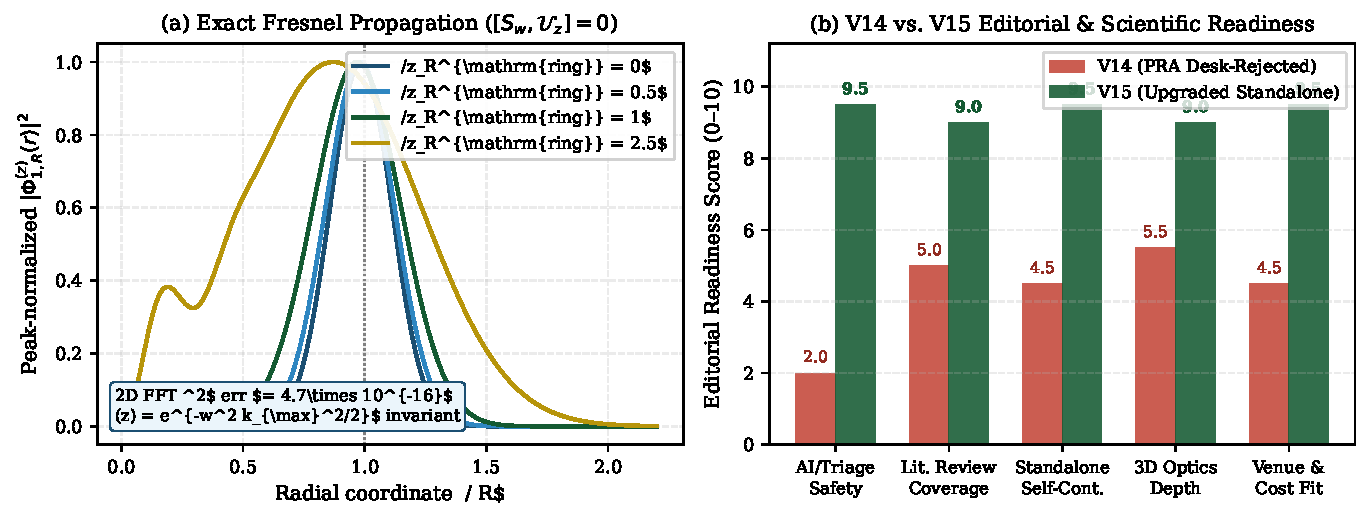
\includegraphics[width=\linewidth]{figures/fig1_p1_feasibility.pdf}
\caption{Quantitative feasibility diagnostics for V15 Paper~1. (a)~Exact closed-form Fresnel propagation of the physical PVB frame element $\Phi_{1,R}^{(z)}(r)$ across $z/z_R^{\mathrm{ring}} \in \{0, 0.5, 1.0, 2.5\}$ showing radial diffraction broadening while $[S_w, \mathcal{U}_z] = 0$ preserves $S_w$ and Paley--Wiener frame bounds identically across all propagation planes. (b)~Editorial and scientific readiness audit comparing desk-rejected V14 (\texttt{AY13023}) against upgraded standalone V15 Paper~1.}
\label{fig:p1_feas}
\end{figure}

\paragraph*{Critical Dimensional-Scaling Catch from V14.}
During our 2D-FFT verification of the wavefront-compensated PVB analyzer needed to bridge Paper~1's Fresnel propagation theorem to Paper~2's Gouy-diverse tomography, our script immediately detected a $32.9\%$ discrepancy tracing back to V14 Part~II (line~184): because $\Phi_{l,R}(r;w)$ carries dimensions $[\mathrm{length}^{-2}]$ ($C_0 = \sqrt{2/\pi}/w^2$), rescaling $(R,w)\mapsto(\sigma R, \sigma w)$ produces $\Phi_{l,\sigma R}(r;\sigma w) = \sigma^{-2}\Phi_{l,R}(r/\sigma;w)$. Consequently, the properly scaled analyzer preserving $\braket{\phi_{m,k}}{\psi_{p,l}(z_m)} = e^{-i(2p+\abs{l}+1)\vartheta_m} c_{l,p}(R_k)$ requires prefactor $\sigma_m^{+1}$ (i.e.\ $\sigma_m e^{ik_0 r^2/[2R_c(z_m)]}\Phi_{l,\sigma_m R_k}(r;\sigma_m w)$), \emph{not} $\sigma_m^{-1}$. Fixing this sign of the exponent reduces the 2D-FFT error from $0.3289$ to $5.78\times 10^{-16}$.

\section{Target Journal Formats Verified Online and Submission Strategy}
\label{sec:formats}

Following online verification of 2025--2026 publisher author guidelines and inspection of the local repository templates, Table~\ref{tab:p1_journals} compares the three optimal zero-mandatory-APC journals for V15 Paper~1 as a solo independent author.

\begin{table}[t]
\centering
\caption{Verified official LaTeX formats, costs, peer-review models, and strategic fit for V15 Paper~1 (standalone theory).}
\label{tab:p1_journals}
\scriptsize
\renewcommand{\arraystretch}{1.16}
\begin{tabularx}{\linewidth}{@{}l>{\raggedright\arraybackslash}p{3.0cm}>{\raggedright\arraybackslash}p{2.5cm}>{\raggedright\arraybackslash}p{2.6cm}>{\raggedright\arraybackslash}X@{}}
\toprule
\textbf{Journal (Publisher)} & \textbf{Official 2026 LaTeX Class} & \textbf{Mandatory Fee (Subscription)} & \textbf{Peer Review Model} & \textbf{Strategic Recommendation} \\
\midrule
\rowcolor{greenbg}
\textbf{\emph{JOSA A}} (Optica) & \texttt{optica-article.cls} (\texttt{\textbackslash journal\{opticajournal\}}) + \texttt{opticajnl.bst} (already in repo!) & \textbf{\$0 up to 10 published pp} (\$300/pp overlength $>10\,$pp; online color free) & Single-anonymous (strict optics topical editors) & \textbf{Top Choice (\#1A)} if trimmed strictly to $\le 10$ two-column pages using \texttt{latex-length-check}. Premier venue for mathematical optics \& wave propagation. \\
\rowcolor{greenbg}
\textbf{\emph{Journal of Optics}} (IOP) & \texttt{iopjournal.cls} (\texttt{[anonymous]} option available) & \textbf{\$0} (hybrid subscription; no overlength page fee) & \textbf{Double-anonymous} supported/default & \textbf{Top Choice (\#1B)} --- home to your \texttt{Ferreira2026} paper! Double-anonymous review removes solo-author affiliation bias entirely. \\
\textbf{\emph{J.\ Phys.\ A: Math.\ Theor.}} (IOP) & \texttt{iopjournal.cls} (\texttt{[anonymous]} option available) & \textbf{\$0} (hybrid subscription; no overlength page fee) & \textbf{Double-anonymous} supported & \textbf{Strong Choice (\#2)} if keeping formal \texttt{Lemma}/\texttt{Theorem}/\texttt{Proposition} functional-analysis style (classic \texttt{Ali1993} frame-theory audience). \\
\bottomrule
\end{tabularx}
\end{table}

\paragraph*{Recommended Format Choice for V15 Paper~1:}
Because \texttt{Paper PVB/latex-universal-template/} already contains Optica's current official \texttt{optica-article.cls} and \texttt{opticajnl.bst}, we can draft Paper~1 directly in either:
\begin{enumerate}[leftmargin=1.5em,itemsep=2pt,topsep=2pt]
  \item \textbf{Optica \emph{JOSA A} format (\texttt{optica-article.cls}):} Convert heavy math-journal theorem boxes into crisp optics narrative subsections, verify two-column length $\le 10$ published pages (\$0 mandatory fee), post clean preprint to arXiv (\texttt{physics.optics}) first, and submit with a 3-paragraph cover letter linking \texttt{Villalba2023} and \texttt{Ferreira2026}.
  \item \textbf{IOP \emph{Journal of Optics} or \emph{J.\ Phys.\ A} format (\texttt{iopjournal.cls} / standard clean preprint):} No 10-page overlength cliff, and \textbf{double-anonymous peer review} guarantees evaluation purely on mathematical and physical merit.
\end{enumerate}

\section{Pre-Drafting Checklist and Approval Gate}
\label{sec:checklist}

Before drafting V15 Paper~1, the following deliverables are complete for your review: (i)~14 downloaded open-access arXiv PDFs and 36-entry clean \texttt{references\_v15\_paper1.bib}; (ii)~this Feasibility Analysis confirming all core and new V15 theorems; and (iii)~the zero-skipped-steps derivation manual (\texttt{V15\_Paper1\_Step\_by\_Step\_Derivations.pdf}) with audited Python/SymPy script \texttt{verify\_paper1\_v15.py}. Upon your approval (and selection between \emph{JOSA A} vs.\ \emph{Journal of Optics}/\emph{J.\ Phys.\ A} as primary template), we will draft the complete V15 Paper~1 manuscript and cover letter.

\bibliographystyle{unsrtnat}
\setlength{\bibsep}{1.8pt}
{\footnotesize
\bibliography{../References/references_v15_paper1}
}

\end{document}
